\documentclass{beamer}

\usepackage[utf8]{inputenc}
\usepackage[francais]{babel}
\usepackage{wrapfig}
\usepackage{amsmath}% http://ctan.org/pkg/amsmath
\usepackage{graphicx}

\usepackage{multirow}

\usepackage{sansmathaccent}
\pdfmapfile{+sansmathaccent.map}
\usepackage{tikz}
\usepackage{verbatim}

\setbeamertemplate{caption}{\raggedright\insertcaption\par}

\usetheme{Singapore}

\title{Détection d'anomalies de classification dans l'IoT via Machine Learning}
\author{Antoine Urban, Yohan Chalier}
\institute{Projet de filière SR2I \\ Télécom ParisTech}

\begin{document}

\begin{frame}
\titlepage
\end{frame}

\section{Introduction}

\begin{frame}{Introduction}
La détection d'obstacles: un enjeu de sécurité !
\begin{figure}
\centering
\includegraphics[width=.8\textwidth]{img/sensors.png}
\caption{Ensemble des capteurs présents dans le véhicule}
\end{figure}
\end{frame}

\begin{frame}{Attaques potentielles}

\begin{columns}

\begin{column}{0.5\textwidth}
\begin{figure}
\centering
\includegraphics[width=\textwidth]{img/blinding.png}
\caption{Attaque par aveuglement des capteurs}
\end{figure}
\end{column}

\begin{column}{0.5\textwidth}
\begin{figure}
\centering
\includegraphics[width=\textwidth]{img/data_flow.png}
\caption{Attaque par modification}
\end{figure}
\end{column}

\end{columns}

\end{frame}


\begin{frame}{Objectifs}
Proposition d'un modèle de classification multi-classes en réalisant un classeur à partir d'un algorithme d'apprentissage supervisé.
\end{frame}

\begin{frame}
\begin{figure}
\centering
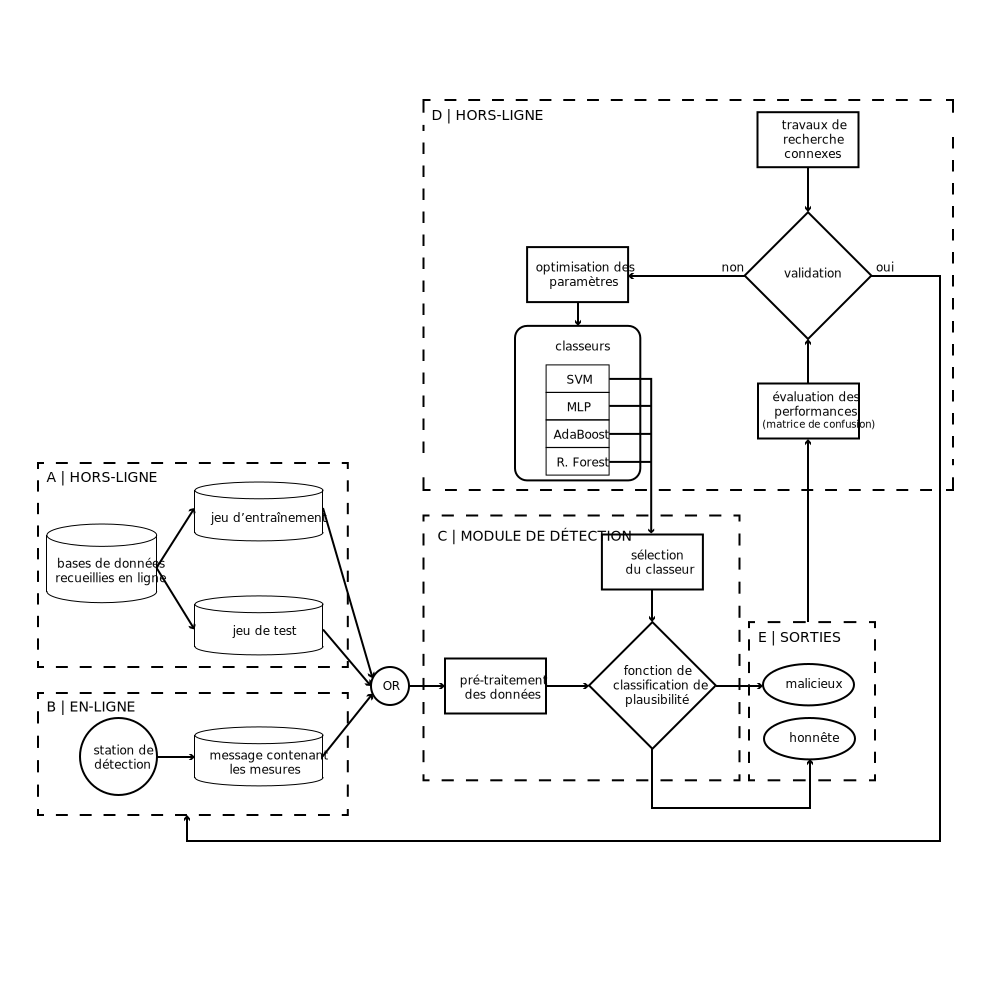
\includegraphics[width=.9\textwidth]{img/structure.png}
\end{figure}
\end{frame}

\section{Démarche de recherche}

\begin{frame}{Première implémentation}
\begin{itemize}
\item Extraction des colonnes largeur et longueur de la base de données
\item Suppression des redondances
\item Définition de zones de décision arbitraires
\item Génération des données malicieuses
\end{itemize}
\begin{table}
\centering
\begin{tabular}{llll}
validité & intervalle de longueur & intervalle de largeur \\
\hline
non-malicieux & 3 à 6,5 mètres & 1,4 à 2,4 mètres \\
malicieux & 3 à 4,1 mètres & 2,05 à 2,4 mètres \\
malicieux & 5,25 à 6,5 mètres & 1,4 à 1,65 mètres \\
\end{tabular}
\end{table}
\end{frame}

\begin{frame}
\begin{figure}
\centering
\includegraphics[width=.8\textwidth]{img/first_try.png}
\end{figure}
\end{frame}

\begin{frame}{Méthodes d'évaluation}
\framesubtitle{Matrice de confusion}

\begin{tabular}{ l | l | c | c | c c}
\multicolumn{2}{c}{} & \multicolumn{2}{c}{Classe réelle} & \\
\cline{3-4}
\multicolumn{2}{c|}{} & Positif & Négatif \\
\cline{2-4}
\multirow{2}{*}{Classe prédite} & Positif & $TP$ & $FP$ & $PPV$ & $FDR$ \\
\cline{2-4}
& Négatif & $FN$ & $TN$ & $FOR$ & $NPV$ \\
\cline{2-4}
\multicolumn{1}{r}{} & \multicolumn{1}{l}{} & \multicolumn{1}{c}{$TPR$} & \multicolumn{1}{c}{$FPR$} \\
\multicolumn{1}{l}{} & \multicolumn{1}{l}{} & \multicolumn{1}{c}{$FNR$} & \multicolumn{1}{c}{$TNR$} \\
\end{tabular}

\end{frame}

\begin{frame}{Chargement des bases de données (1/2)}

\begin{enumerate}
\item Pour chaque jeu de données au format CSV
\begin{enumerate}[{1.}1.]
\item Lire les colonnes contenant la longueur et la largeur
\item Renommer ces colonnes en "\texttt{length}" et "\texttt{width}"
\item Supprimer les lignes incomplètes
\item Si nécessaire, convertir les données en flottant et en millimètres
\item Ajouter une colonne contenant la classe correspondant au jeu de données considéré
\item Appliquer un premier filtre sur la longueur ou la largeur pour supprimer les points extrêmes isolés
\end{enumerate}
\item Fusionner toutes les matrices précédentes en une seule
\item Créer un nouvel objet \texttt{Detector} avec cette matrice en attribut
\end{enumerate}

\end{frame}

\begin{frame}{Chargement des bases de données (2/2)}
\begin{enumerate}
\item Supprimer les éventuels redondances
\item Ajouter une colonne "\texttt{odd}" à la matrice, initialisée à \texttt{False}
\item \textbf{Générer les données malicieuses}
\item Ajouter les données malicieuses à la base de données, en rajoutant la colonne "\texttt{odd}" initialisée à \texttt{True}
\item Remplacer les valeurs des classes (originnellement des chaînes de caractères comme \texttt{"car"} ou \texttt{"human"}) par des entiers
\item \textbf{Séparer la matrice en un jeu d'entraînement et un jeu de test}
\item Renvoyer l'objet \texttt{Detector} ainsi initialisé
\end{enumerate}
\end{frame}

\begin{frame}{Classe \texttt{Detector}}
\begin{itemize}
\item Pré-traitement \begin{itemize}
\item \texttt{clean}
\item \texttt{append\_odd\_points}
\item \texttt{format}
\end{itemize}
\item Interface scikit-learn \begin{itemize}
\item \texttt{classify}
\item \texttt{tune\_parameters}
\item \texttt{predict}
\end{itemize}
\item Affichage \begin{itemize}
\item \texttt{plot}
\item  \texttt{plot\_decision\_boudaries}
\end{itemize}
\end{itemize}
\end{frame}

\begin{frame}{Méthodes d'évaluation}
\framesubtitle{Score F1}

\begin{block}{Objectif}
Maximisation du score F1 comme critère de performance
\end{block}

\begin{equation}
\text{f1-score} = \dfrac{2\times(\text{Recall} \times \text{Precision})}{(\text{Recall} + \text{Precision})} = 2\times\dfrac{PPV \times TPR}{PPV + TPR}
\end{equation}

\begin{equation}
\text{Precision} = \dfrac{TP}{TP+FP}
\end{equation}

\begin{equation}
\text{Recall} = \dfrac{TP}{TP+FN}
\end{equation}

\end{frame}

\section{Paramétrage et résultats}

\begin{frame}{Recherche exhaustive et validation croisée}
\begin{itemize}
\item Tests des jeux de paramètres optimaux via la fonction de scikit-learn \texttt{GridSearchCV}
\item Utilise la validation croisée
\item Utilisation d'une fonction de score personnalisée \begin{enumerate}
\item Classification des éléments du jeu de test
\item Calcul de la matrice de confusion
\item Sauvegarde des paramètres et du score
\item Retour du \emph{f1-score}
\end{enumerate}
\item Export des données en formats exploitables (JSON, CSV)
\end{itemize}
\end{frame}

\begin{frame}{Paramètres optimaux}
\framesubtitle{Perceptron à couches multiples}

\begin{table}
\tiny
\centering
\begin{tabular}{l l}
paramètre & ensemble des valeurs testées \\
\hline
\texttt{learning\_rate} & \texttt{'constant'}, \texttt{'invscaling'} et \texttt{'adaptive'}\\
\texttt{alpha} & $\{10^{-k} \>\> | \>\> k \in [\![4, 7]\!] \}$ \\
\texttt{activation} & \texttt{'identity'}, \texttt{'logistic'}, \texttt{'tanh'} et \texttt{'relu'}\\
\texttt{solver} &\texttt{'lbfgs'}, \texttt{'sgd'} et \texttt{'adam'} \\
\texttt{hidden\_layer\_sizes} & 0 à 5 \emph{layers}, de taille variant de 1 à 49 \\
\end{tabular}
\end{table}

\begin{table}
\centering
\begin{tabular}{l l}
paramètre & valeur optimale \\
\hline
\texttt{learning\_rate} & \texttt{'constant'}\\
\texttt{alpha} & $10^{-6}$ \\
\texttt{activation} & \texttt{'tanh'}\\
\texttt{solver} & \texttt{'lbfgs'}\\
\texttt{hidden\_layer\_sizes} & \texttt{[28, 28, 28]}\\
\end{tabular}
\end{table}

\end{frame}

\begin{frame}
\begin{figure}
\centering
\includegraphics[width=.7\textwidth]{img/mlp_activation.png}
\end{figure}
\end{frame}

\begin{frame}{Paramètres optimaux}
\framesubtitle{AdaBoost}
\begin{table}
\tiny
\centering
\begin{tabular}{l l}
paramètre & ensemble des valeurs testées \\
\hline
\texttt{n\_estimators} & $[\![1, 99]\!]$ \\
\texttt{learning\_rate} & $\{k/10 \>\> | \>\> k \in [\![1, 9]\!] \}$ \\
\texttt{base\_estimator} & Arbres de décision de profondeur maximale dans $[\![2, 9]\!]$ \\
\end{tabular}
\end{table}

\begin{table}
\centering
\begin{tabular}{l l}
paramètre & valeur optimale \\
\hline
\texttt{n\_estimators} & 46\\
\texttt{learning\_rate} & 0.3 \\
\texttt{base\_estimator} & \texttt{max\_depth=}3\\
\end{tabular}
\end{table}

\end{frame}

\begin{frame}
\begin{figure}
\centering
\includegraphics[width=.7\textwidth]{img/adaboost_depth.png}
\end{figure}
\end{frame}

\begin{frame}{Performances des classeurs}
\begin{table}
\centering
\begin{tabular}{r | llllll}
& \emph{TPR} & \emph{FPR} & \emph{TNR} & \emph{FNR} & \emph{PPV} & \emph{f1-score} \\ 
MLP & 0.568 & 0.005 & 0.995 & 0.432 & 0.949 & 0.711 \\
AdaBoost & 0.935 & 0.010 & 0.990 & 0.065 & 0.941 & 0.938 \\
SVM & 0.966 & 1.0 & 0.0 & 0.034 & 0.145 & 0.252 \\
R. Forest & 0.917 & 0.007 & 0.993 & 0.083 & 0.960 & 0.938 \\
\end{tabular}
\end{table}
\end{frame}

\begin{frame}{Régions de décision}
\begin{figure}
\centering
\includegraphics[width=.65\textwidth]{img/adaboost_contour.png}
\end{figure}
\end{frame}

\begin{frame}{Prédiction en ligne}
\begin{enumerate}
\item Créer un objet \texttt{Detector} en chargeant les bases de données récoltées
\item Entraîner un classeur, dont les paramètres sont ceux résultant de l'optimisation effectuée précédemment, avec ces données
\item Attribuer ce classeur en tant que classeur de prédiction pour le \texttt{Detector}
\item Sauvegarder la méthode \texttt{predict}
\end{enumerate}
\end{frame}


\end{document}
